\documentclass[11pt]{article}
\usepackage[margin=1in]{geometry}
\usepackage{booktabs}
\usepackage{graphicx}
\usepackage{float}
\begin{document}
\section*{Supplementary Step 5 Visualization Report}
\subsection*{Overview}
\begin{tabular}{p{0.36\linewidth}p{0.54\linewidth}}
\toprule
Metric & Value\\
\midrule
Representative geometry session & PID001 / 2025-11-06\_008\\
Included participant-sessions from Step 5 & 36\\
Abstract onset-locked epochs used & 539\\
Concrete onset-locked epochs used & 536\\
Epoch window & -3.5 s to 13.2 s around question onset\\
Baseline & -2.0 s to 0.0 s\\
Primary fixed window & 7.0 s to 11.0 s\\
Long-channel montage used in descriptive plots & 22 pairs (44 chromophore channels)\\
Condition mapping for adapted examples & Abstract versus Concrete\\
\bottomrule
\end{tabular}
\paragraph{Adaptation note.} The reference examples were written for a motor task with Tapping, Control, Left, and Right conditions. For the present experiment, those plot families were adapted to the two available task conditions, Abstract and Concrete. All descriptive response-consistency and topographic plots in this report use the Step~5 long-channel montage so that the visualization set stays aligned with the fixed-window ROI analysis.
\paragraph{Rendering note.} As in the Step~4 supplementary visualization report, the sensor-geometry figure uses the participant digitization point cloud plus source, detector, channel, and pair geometry rather than an fsaverage brain-surface rendering, because the local \texttt{pyvista}/\texttt{fsaverage} stack is not available in this environment.
\subsection*{Step 5 Main Figures Reused}
\begin{figure}[H]
\centering
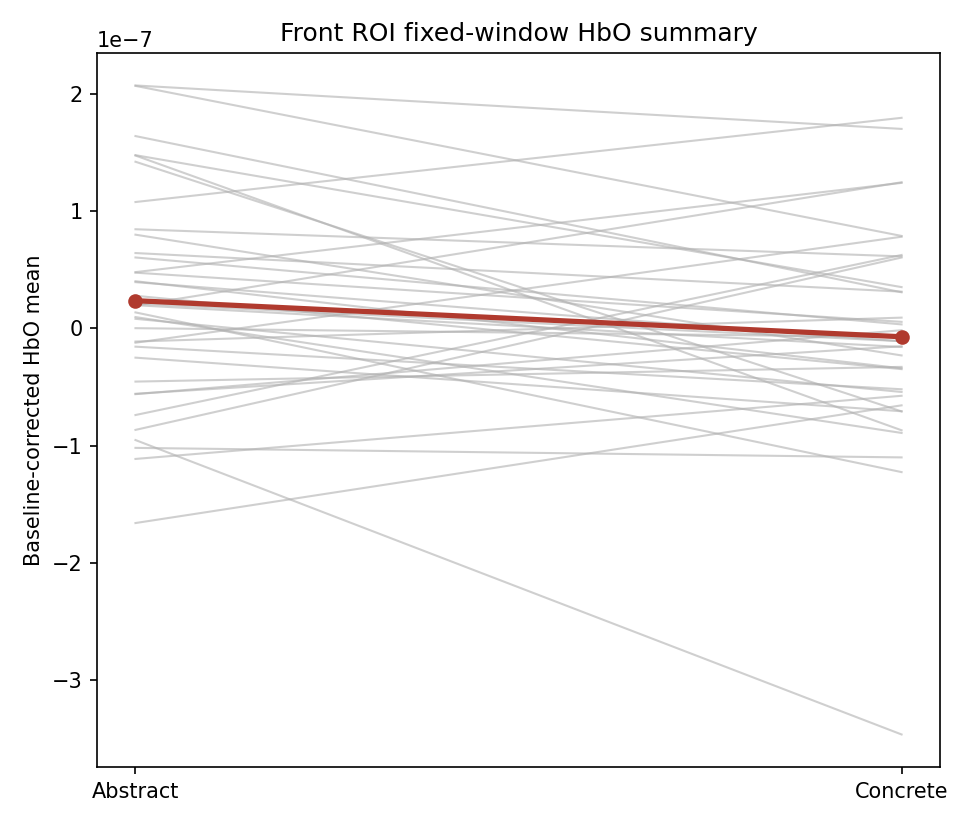
\includegraphics[width=0.48\linewidth]{../../figures/step5/front_roi_window_plot.png}
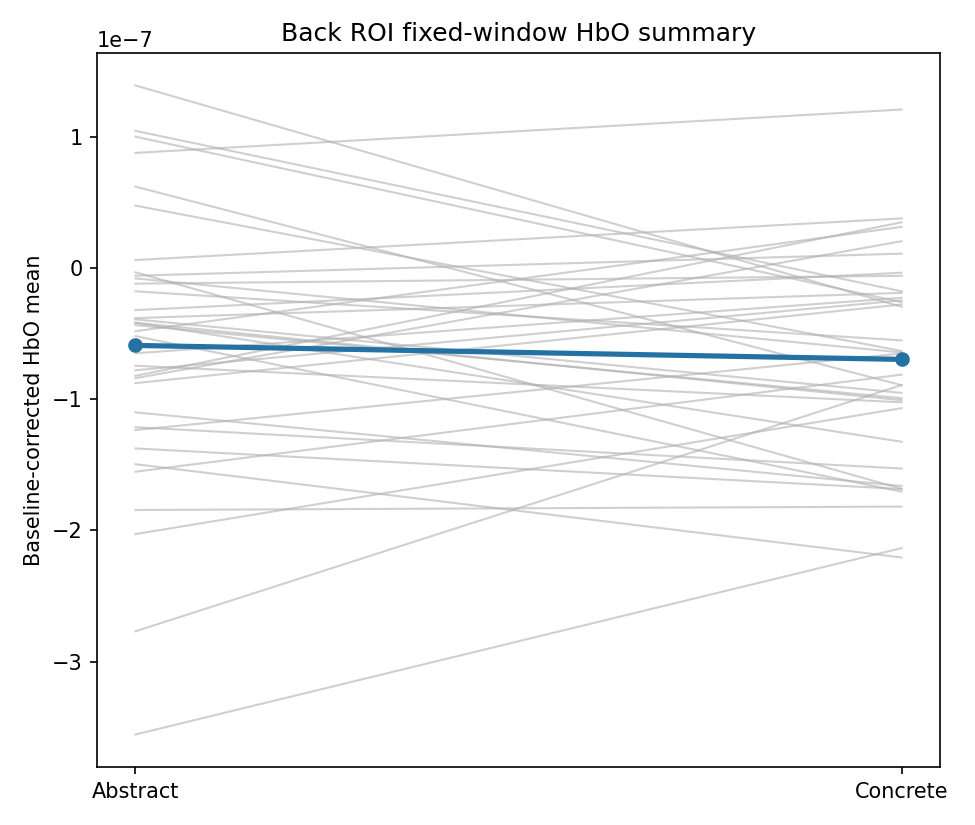
\includegraphics[width=0.48\linewidth]{../../figures/step5/back_roi_window_plot.png}
\caption{Participant-level fixed-window HbO summaries for the front and back ROIs from the main Step~5 report.}
\end{figure}
\begin{figure}[H]
\centering
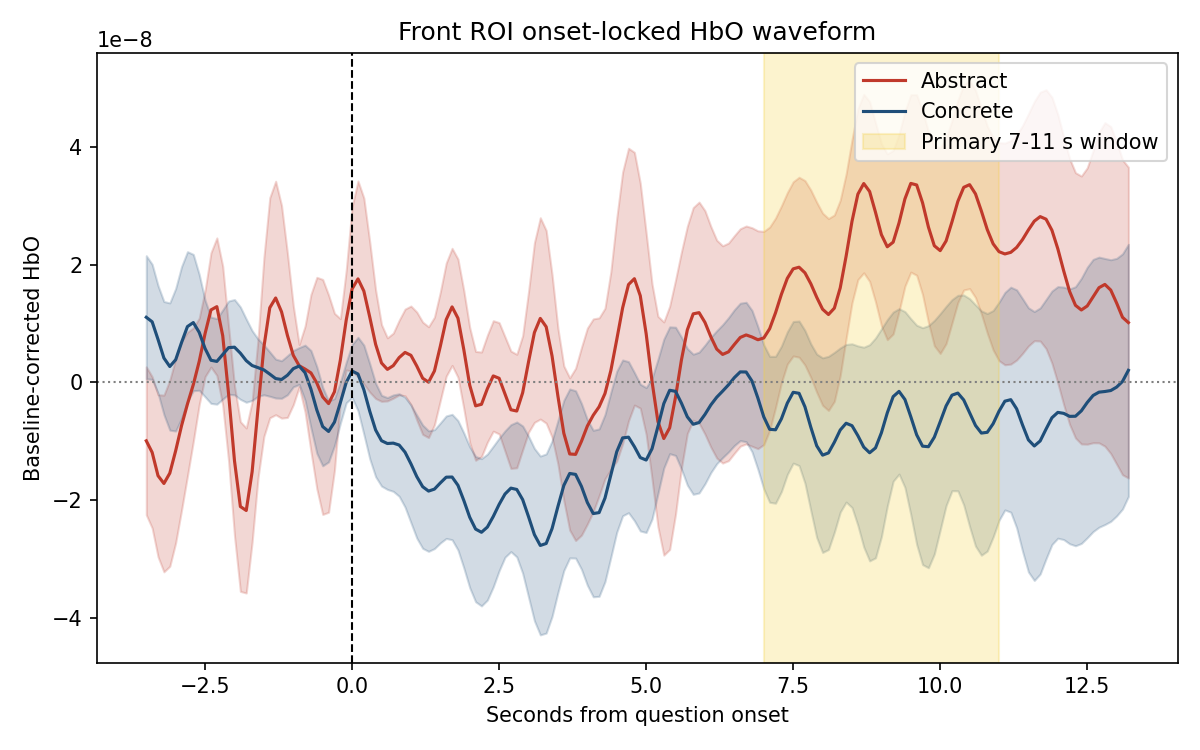
\includegraphics[width=0.48\linewidth]{../../figures/step5/front_waveform_with_window.png}
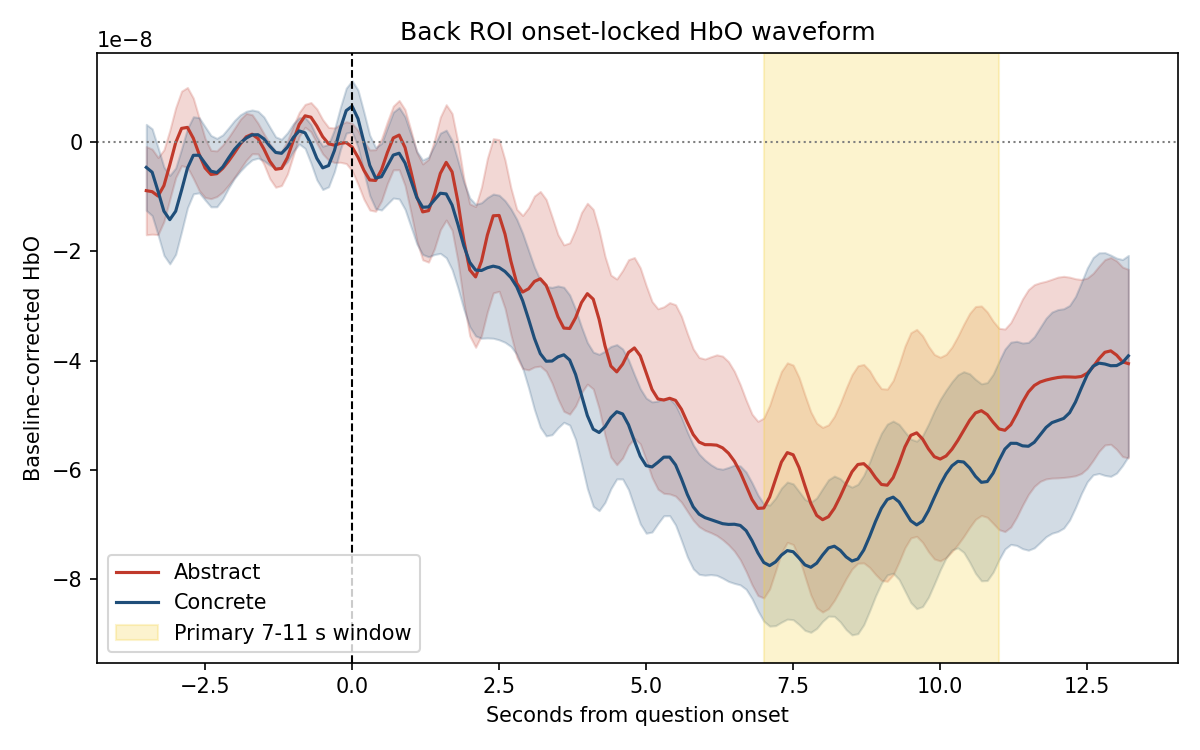
\includegraphics[width=0.48\linewidth]{../../figures/step5/back_waveform_with_window.png}
\caption{Step~5 onset-locked HbO waveforms with the primary 7--11~s analysis window shaded.}
\end{figure}
\begin{figure}[H]
\centering
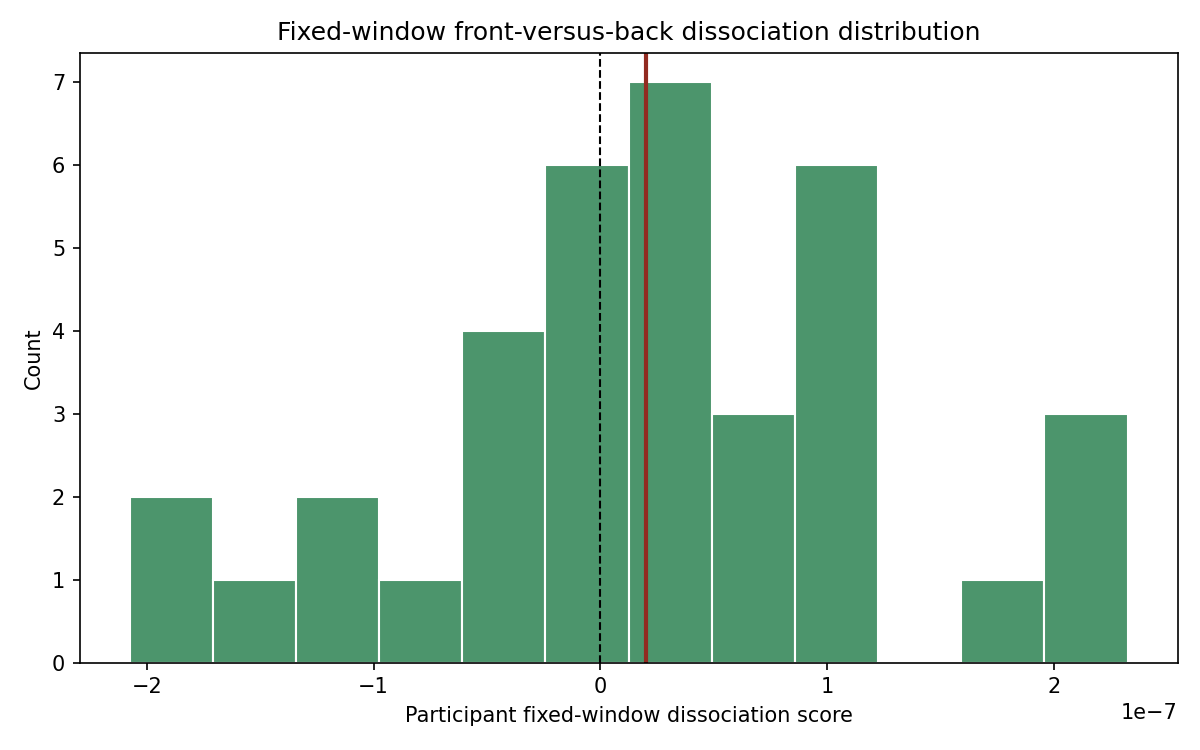
\includegraphics[width=0.48\linewidth]{../../figures/step5/dissociation_histogram_fixed_window.png}
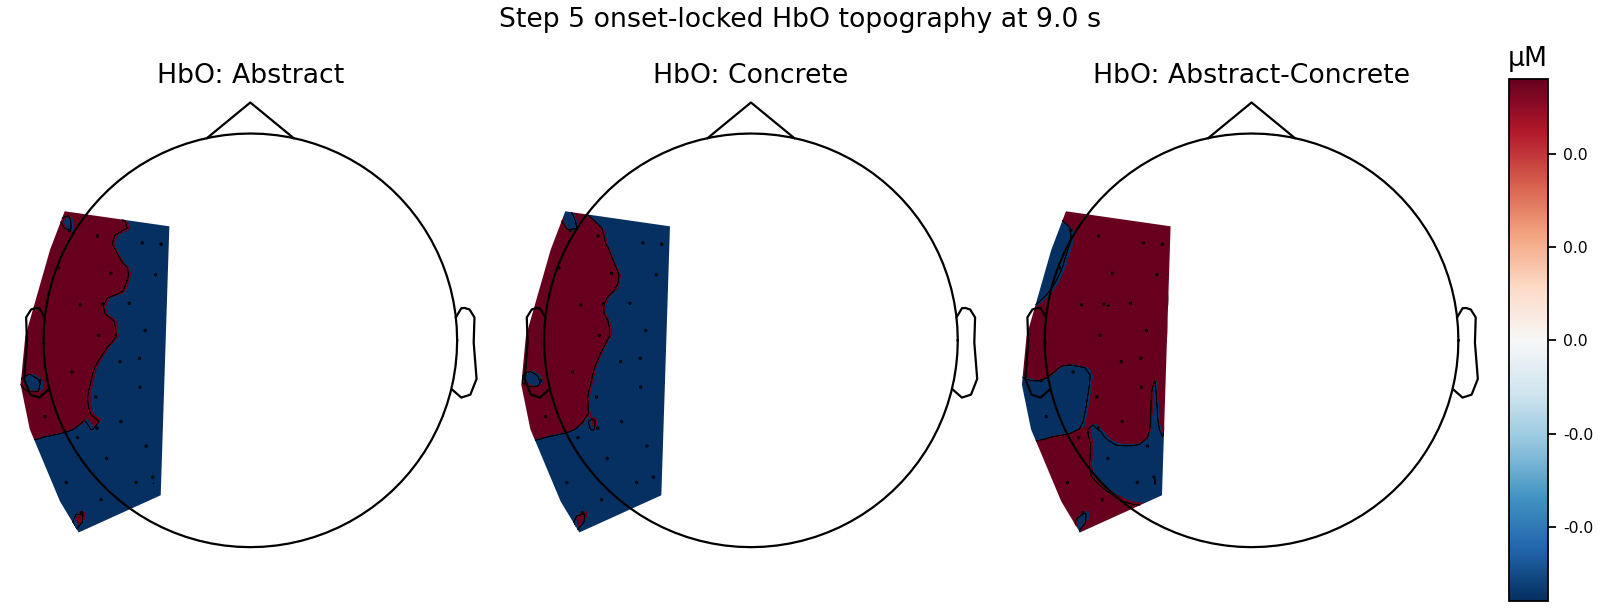
\includegraphics[width=0.48\linewidth]{../../figures/step5/topography_9s.png}
\caption{Fixed-window dissociation histogram and the Step~5 single-time HbO topography at 9.0~s.}
\end{figure}
\subsection*{Sensor Geometry}
\begin{figure}[H]
\centering
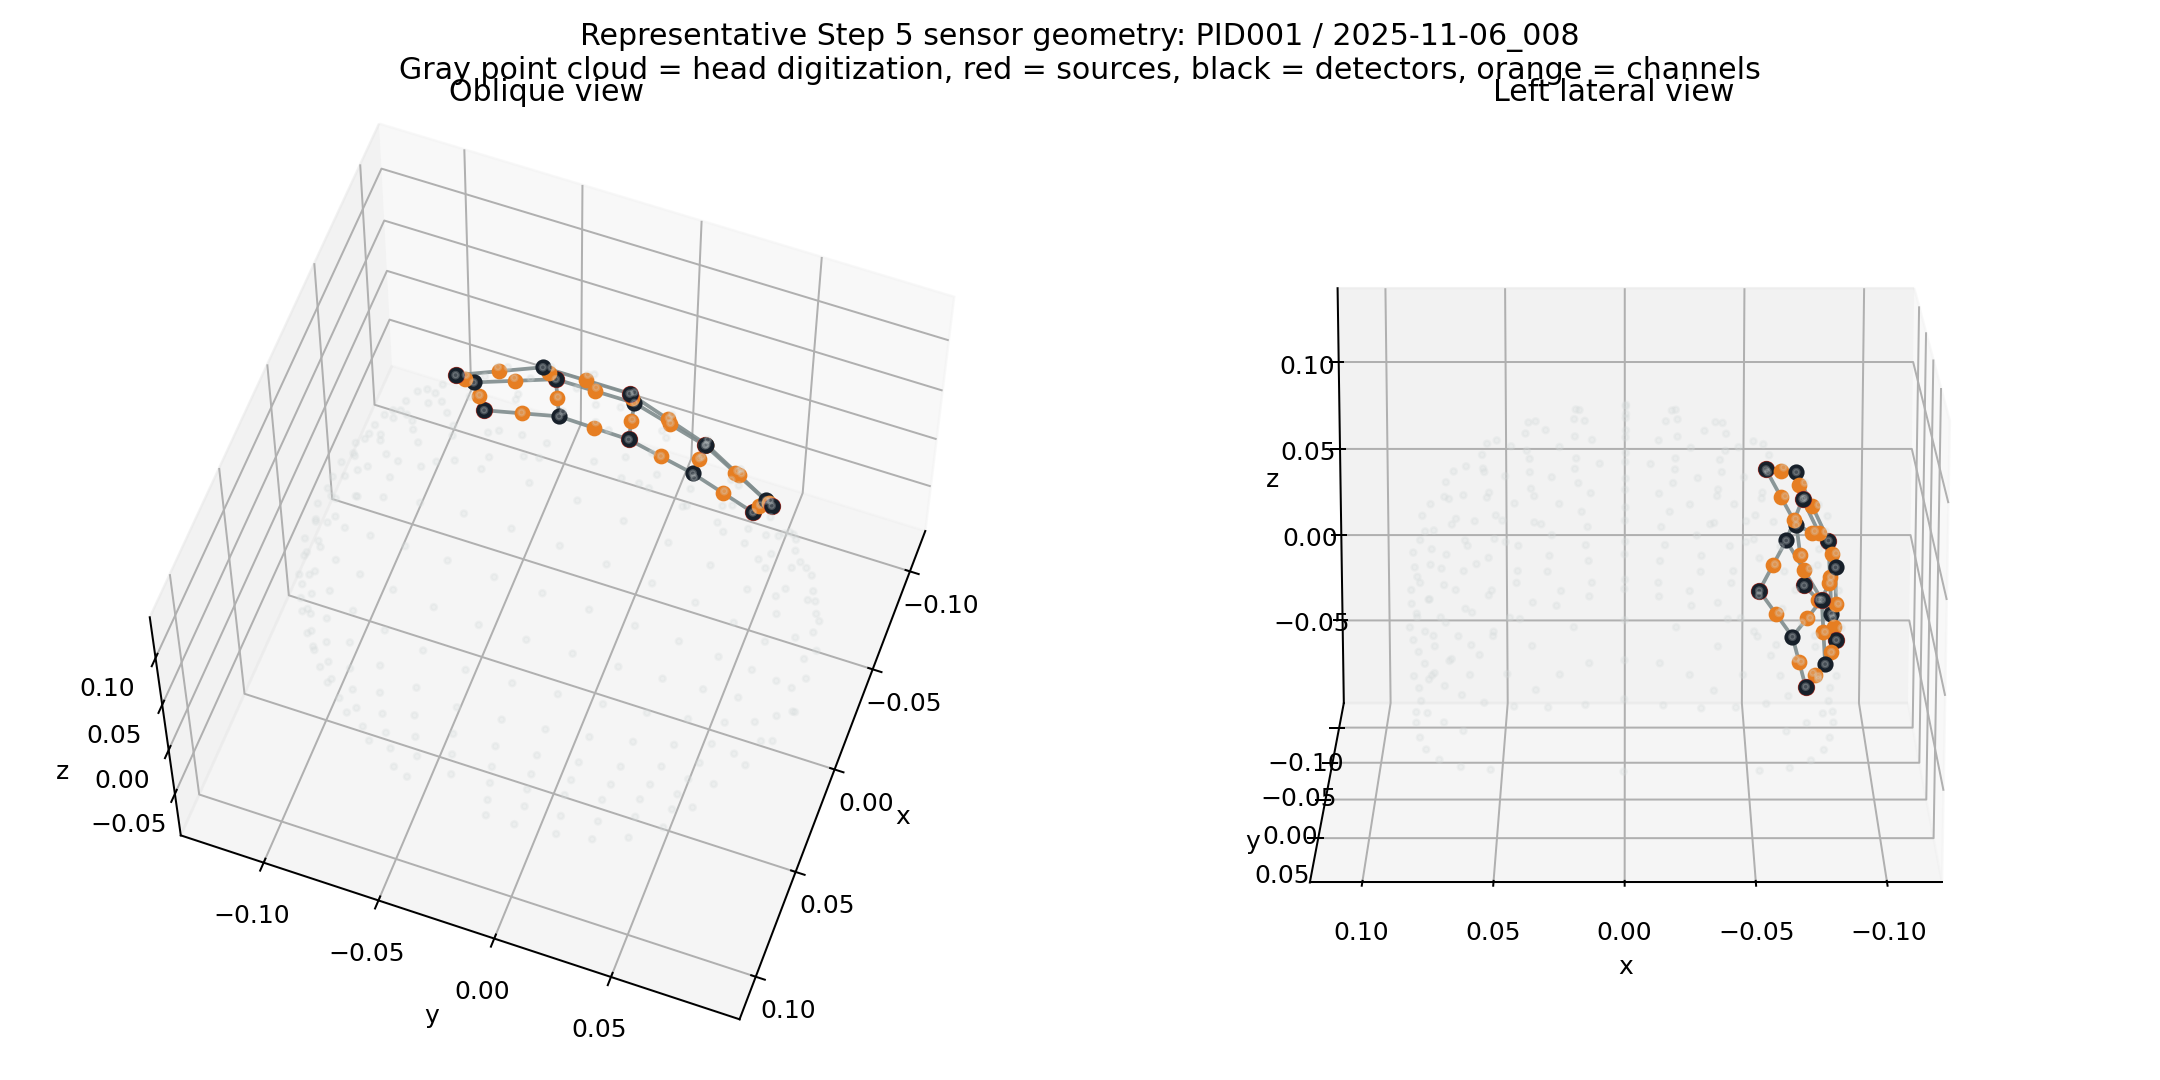
\includegraphics[width=0.95\linewidth]{../../figures/step5_visualization/representative_sensor_geometry.png}
\caption{Representative optode, channel, and source-detector-pair geometry for one Step~5 included participant-session. Short pairs are shown with dashed orange lines.}
\end{figure}
\subsection*{Consistency Across Trials}
\begin{figure}[H]
\centering
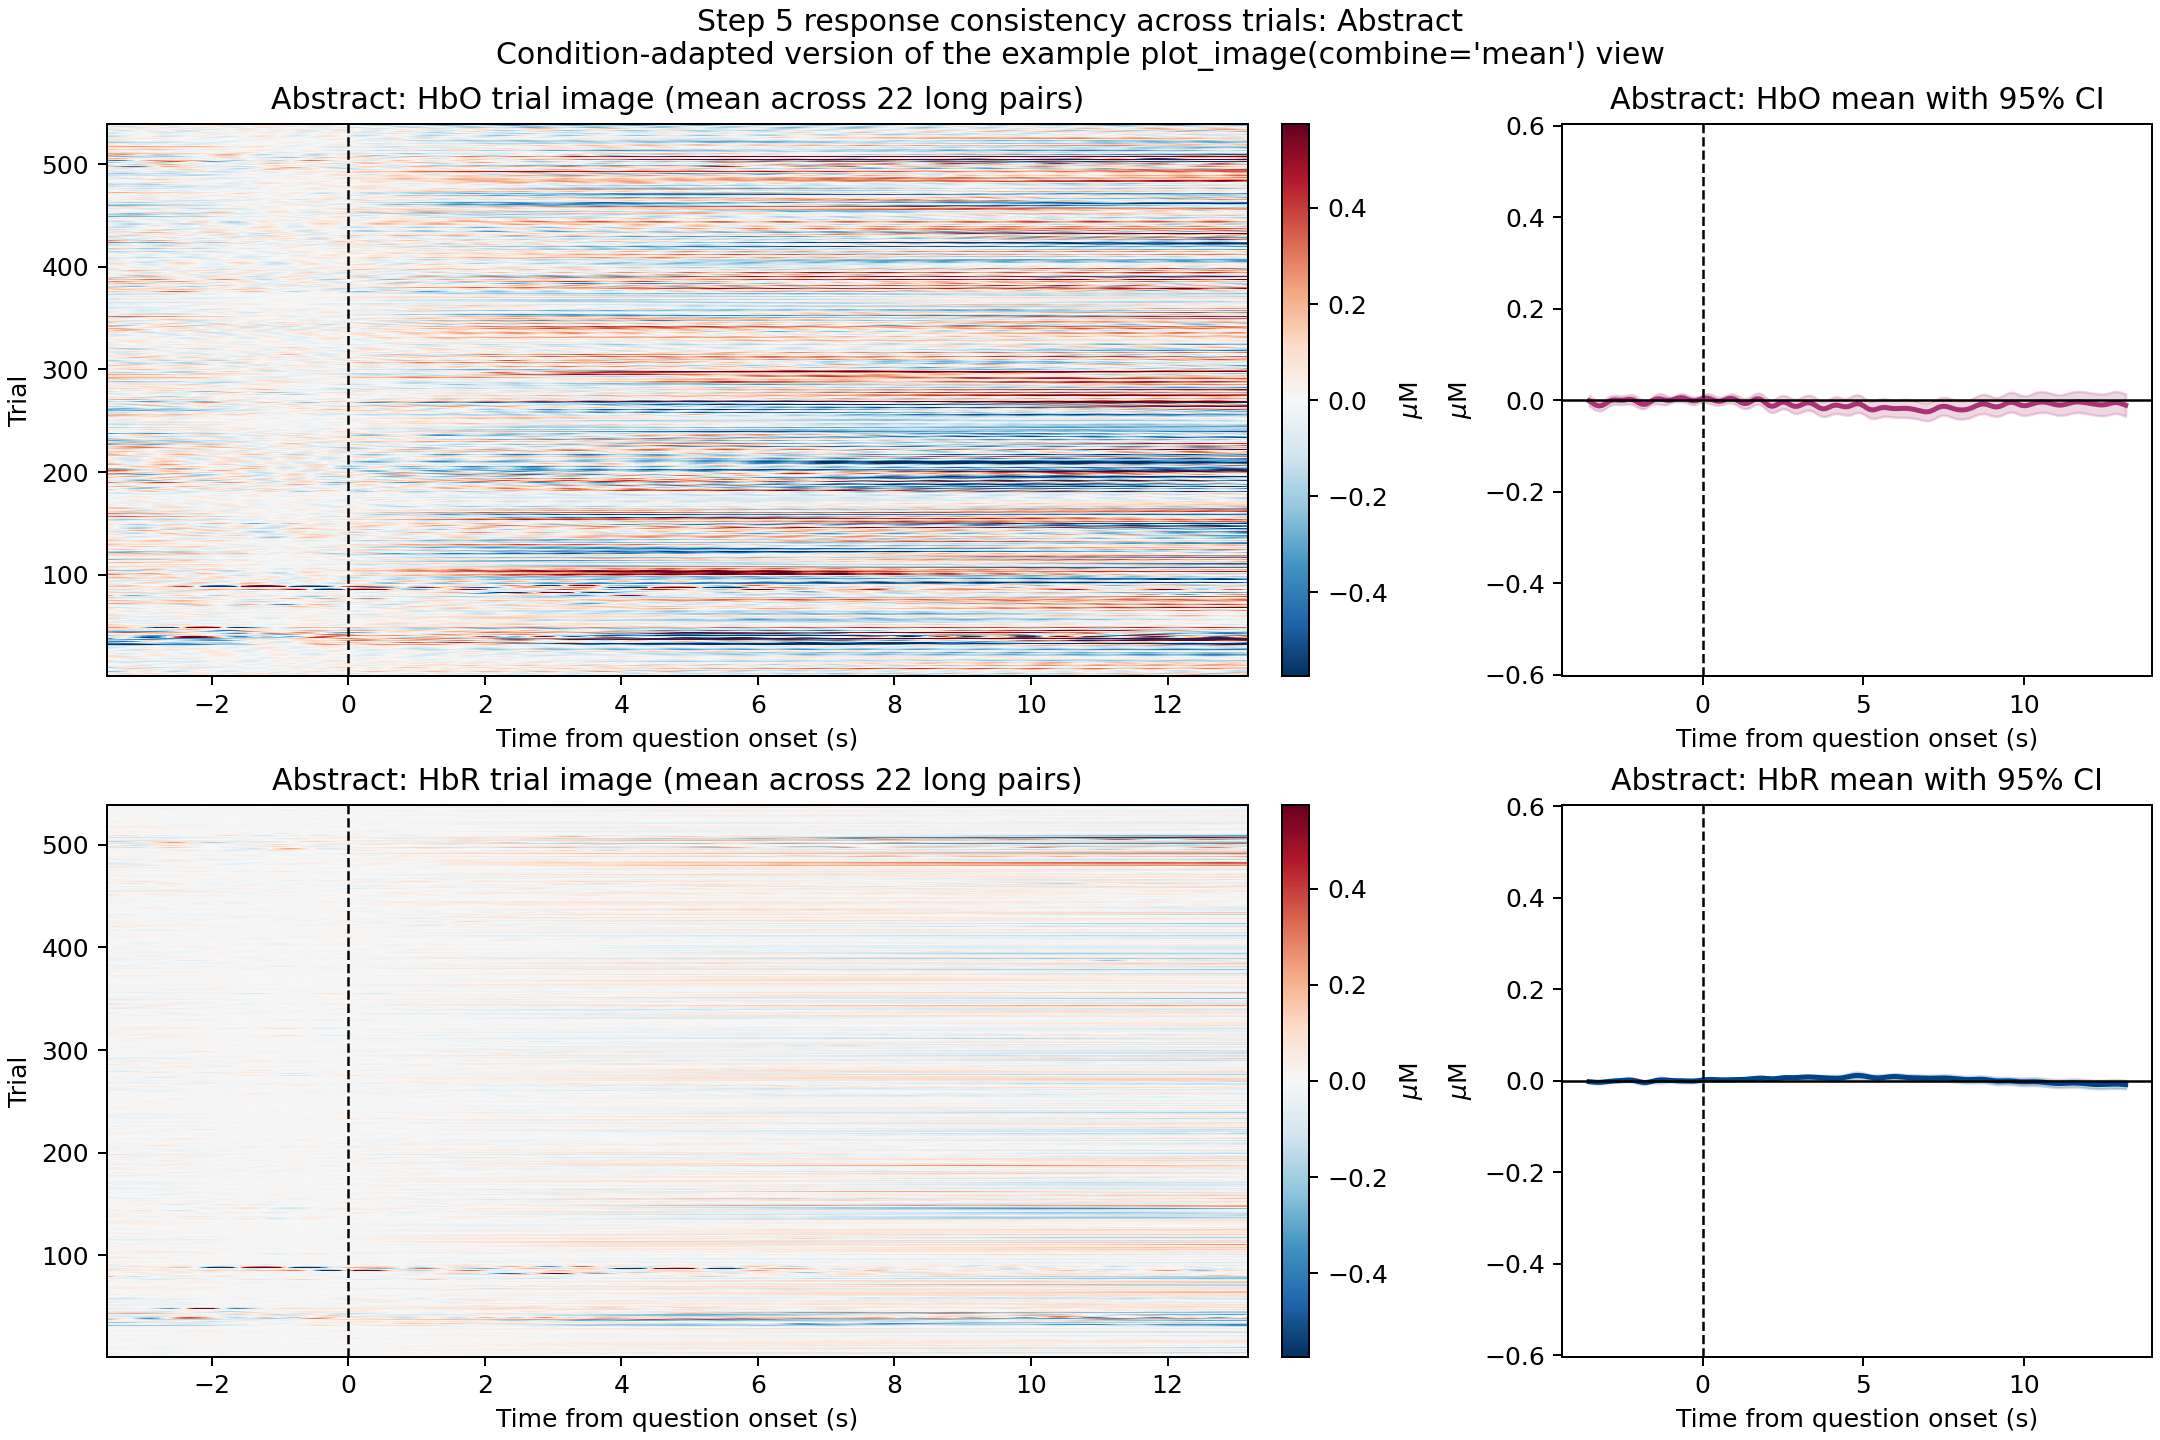
\includegraphics[width=0.48\linewidth]{../../figures/step5_visualization/abstract_trial_consistency.png}
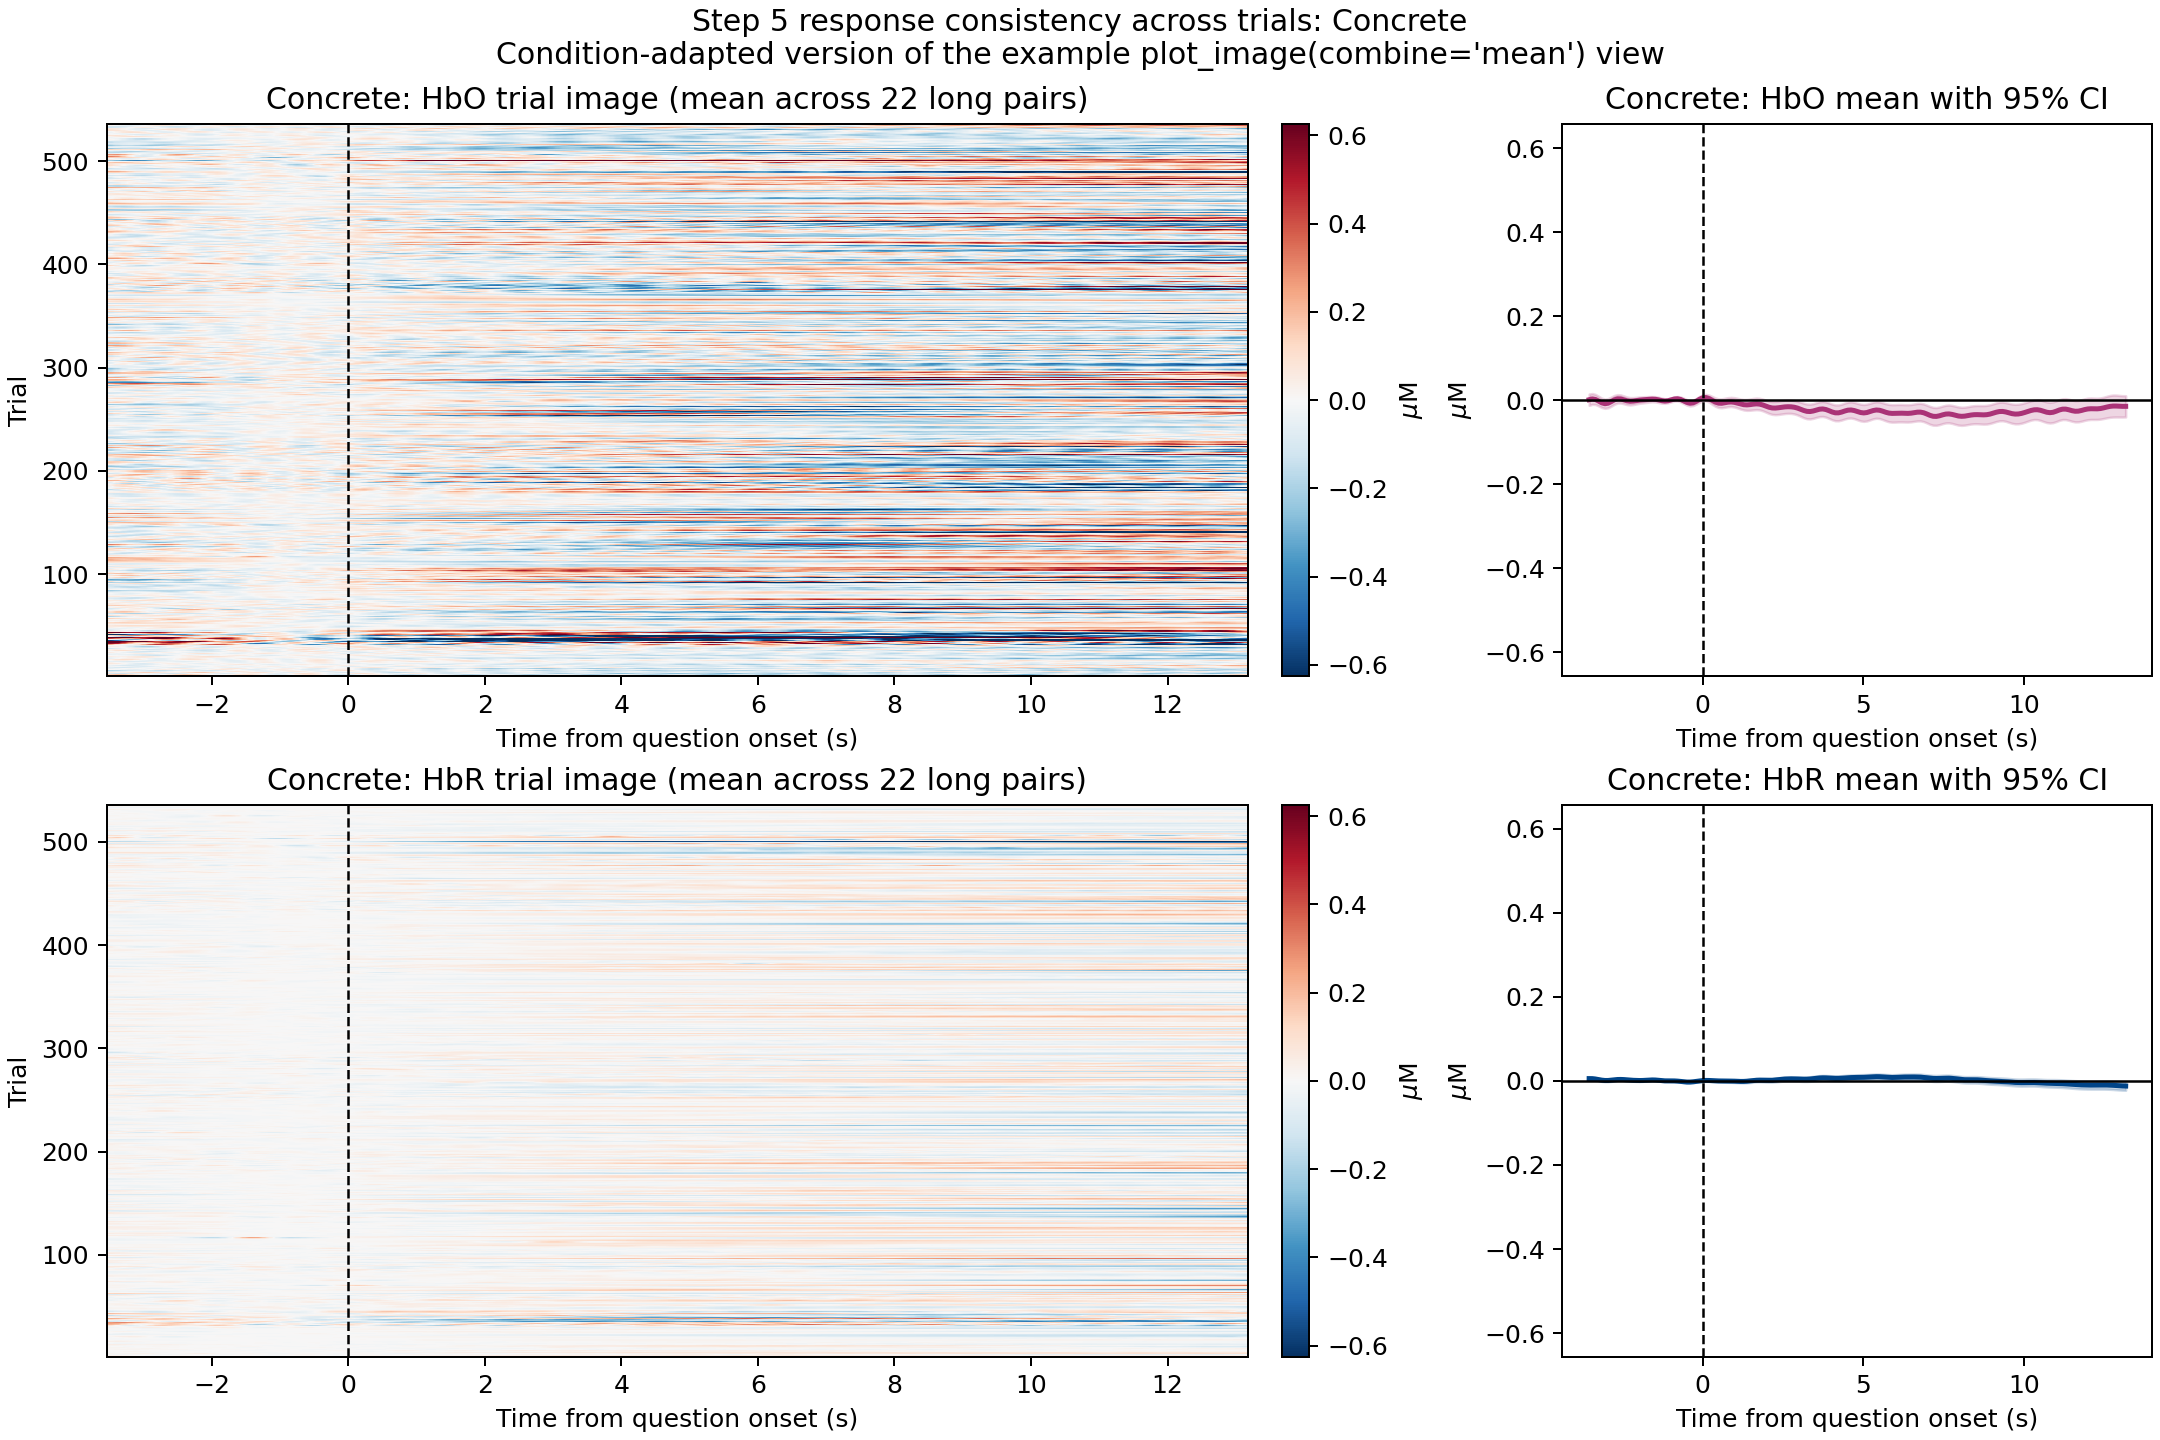
\includegraphics[width=0.48\linewidth]{../../figures/step5_visualization/concrete_trial_consistency.png}
\caption{Condition-adapted versions of the trial-consistency image plots. Each panel shows the mean long-channel HbO and HbR response across individual trials for Abstract and Concrete questions separately.}
\end{figure}
\subsection*{Consistency Across Channels}
\begin{figure}[H]
\centering
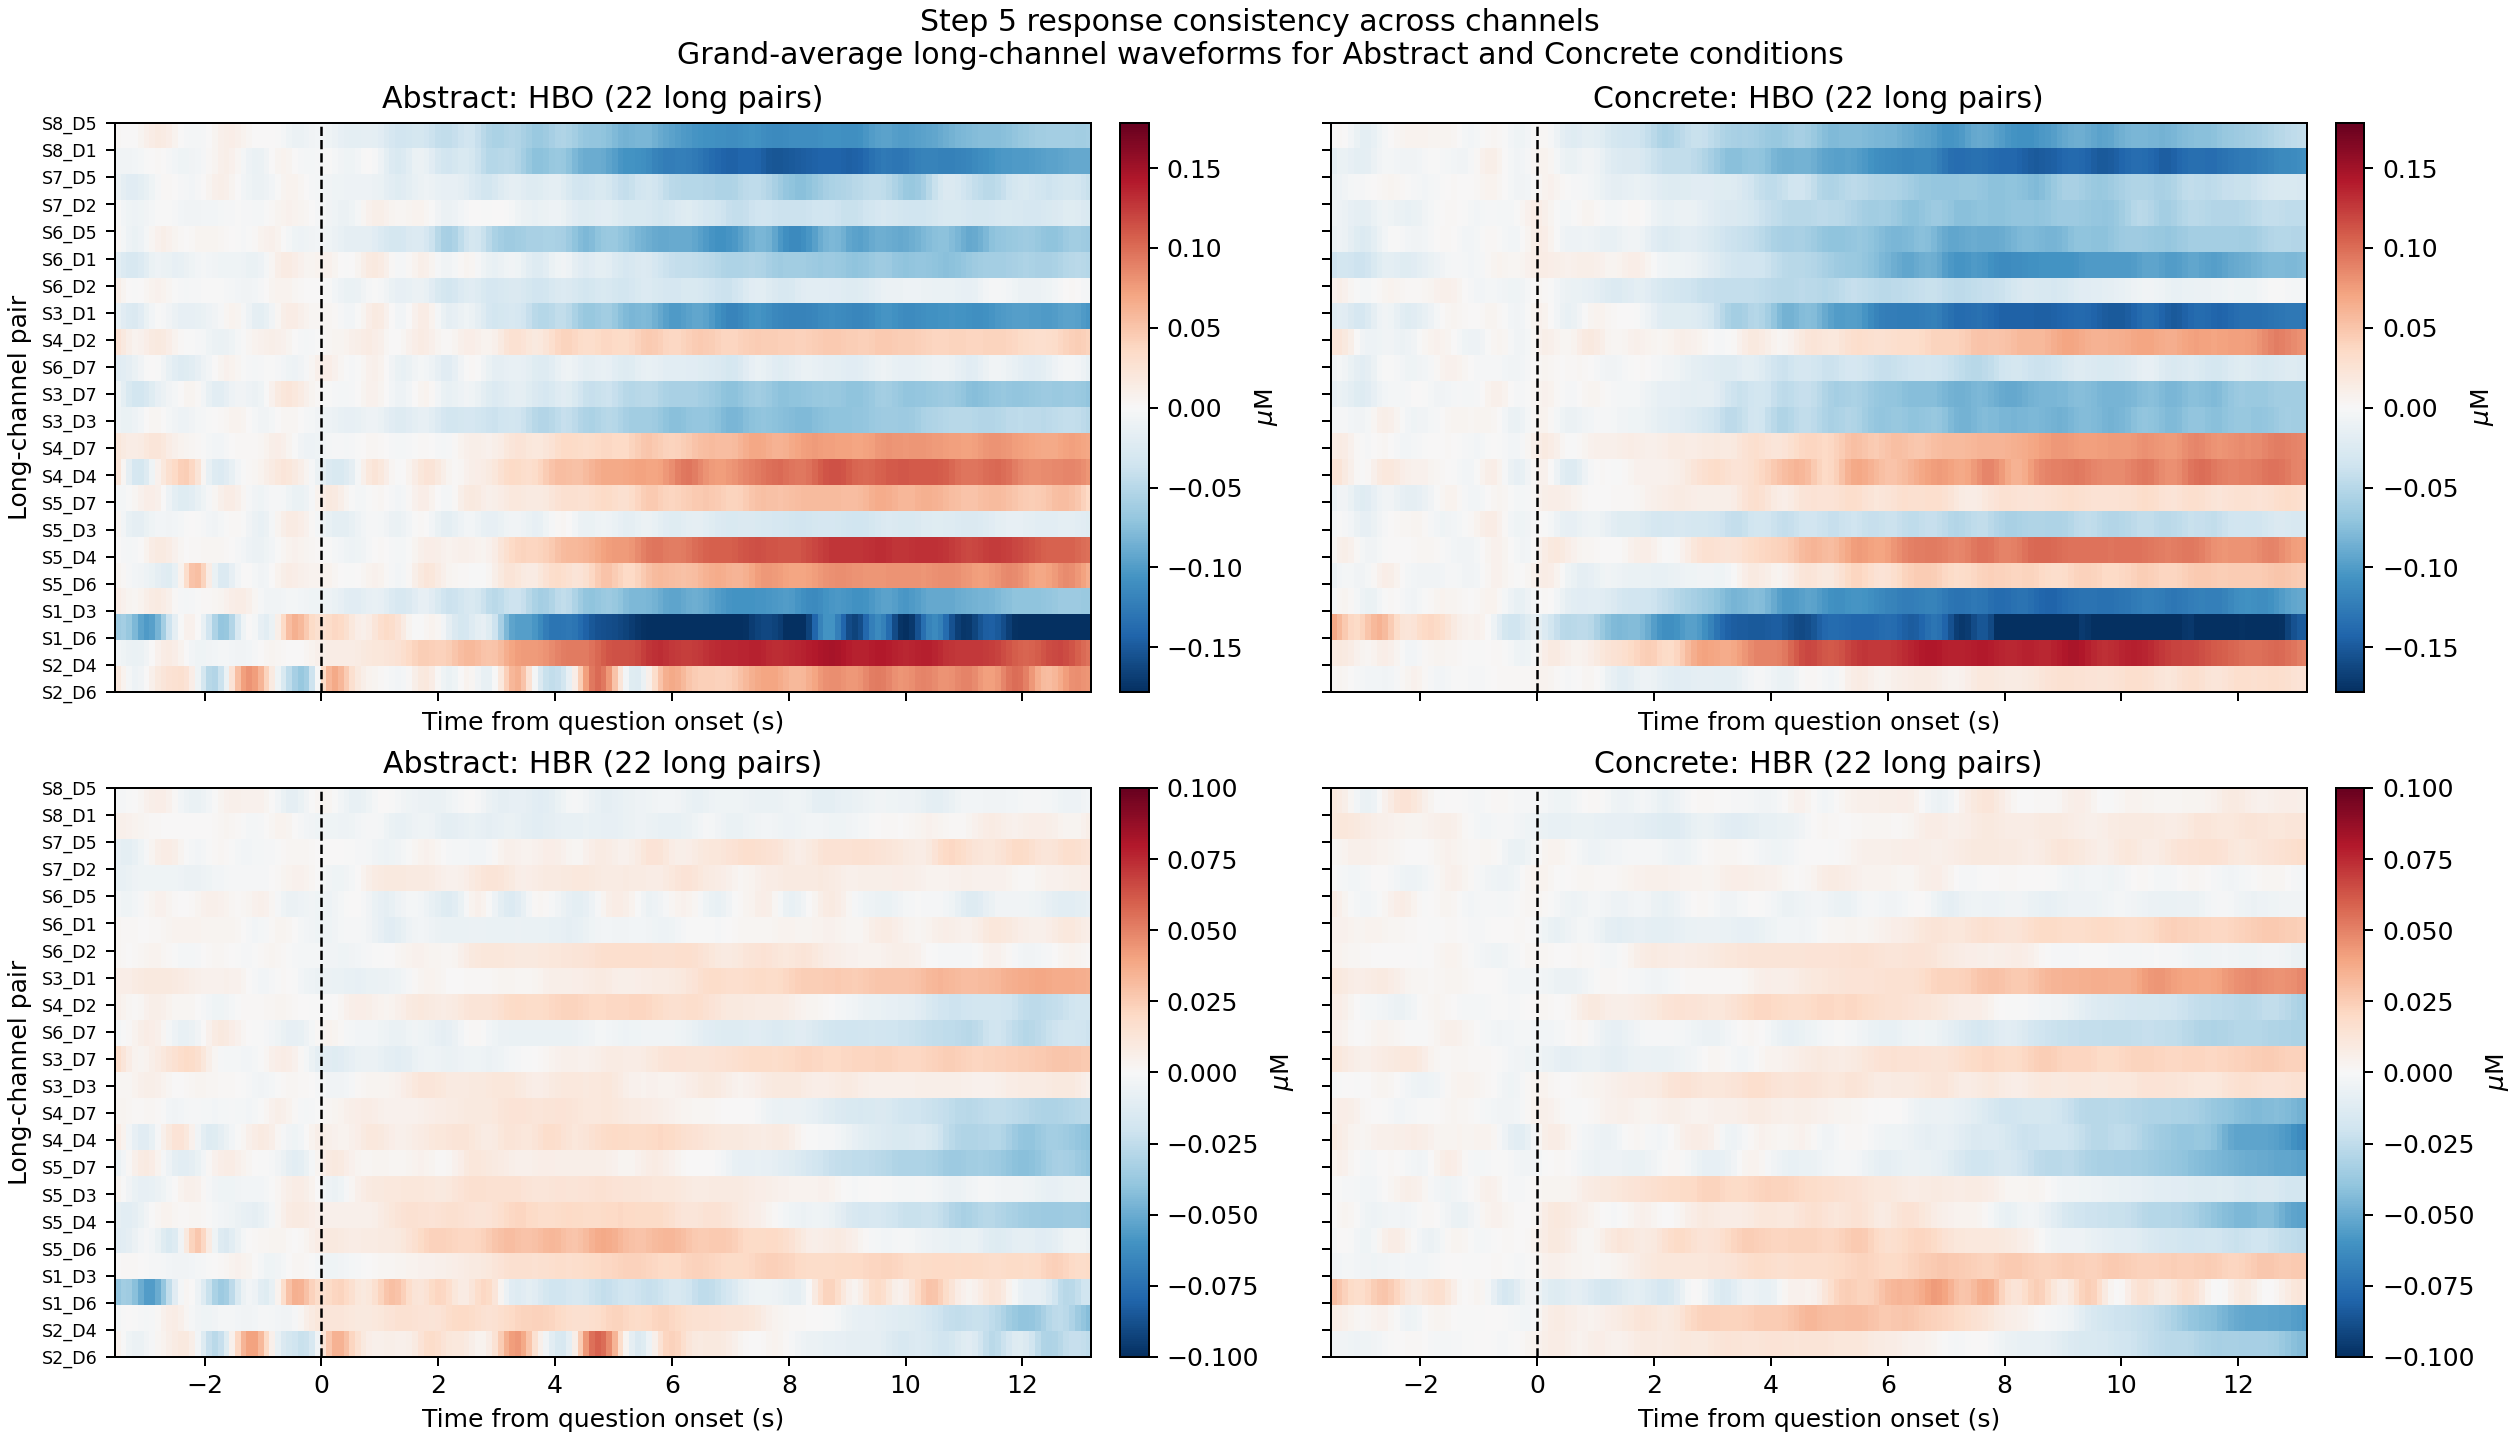
\includegraphics[width=0.95\linewidth]{../../figures/step5_visualization/channel_consistency_grid.png}
\caption{Grand-average long-channel response images across channels for the Abstract and Concrete conditions. Rows correspond to HbO and HbR, and columns correspond to the two conditions.}
\end{figure}
\subsection*{Standard fNIRS Waveform Summary}
\begin{figure}[H]
\centering
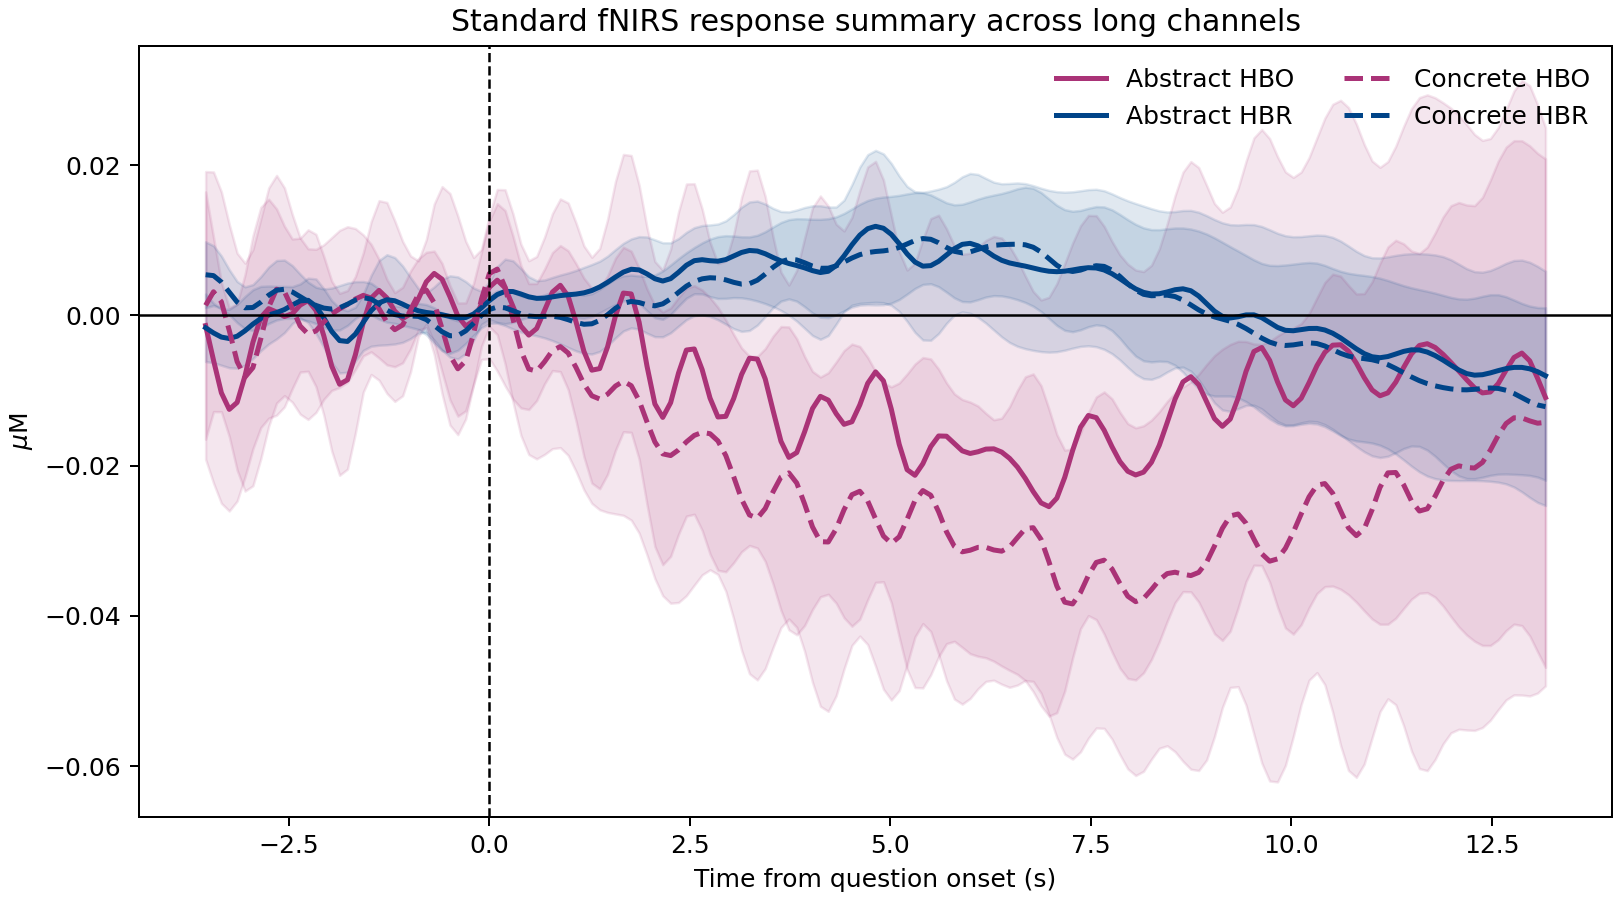
\includegraphics[width=0.92\linewidth]{../../figures/step5_visualization/standard_fnirs_compare.png}
\caption{Condition-adapted standard fNIRS waveform plot. Solid lines indicate Abstract, dashed lines indicate Concrete, magenta shows HbO, and blue shows HbR. Shaded bands show 95\% confidence intervals across participant-sessions.}
\end{figure}
\subsection*{Topographic Representation Over Time}
\begin{figure}[H]
\centering
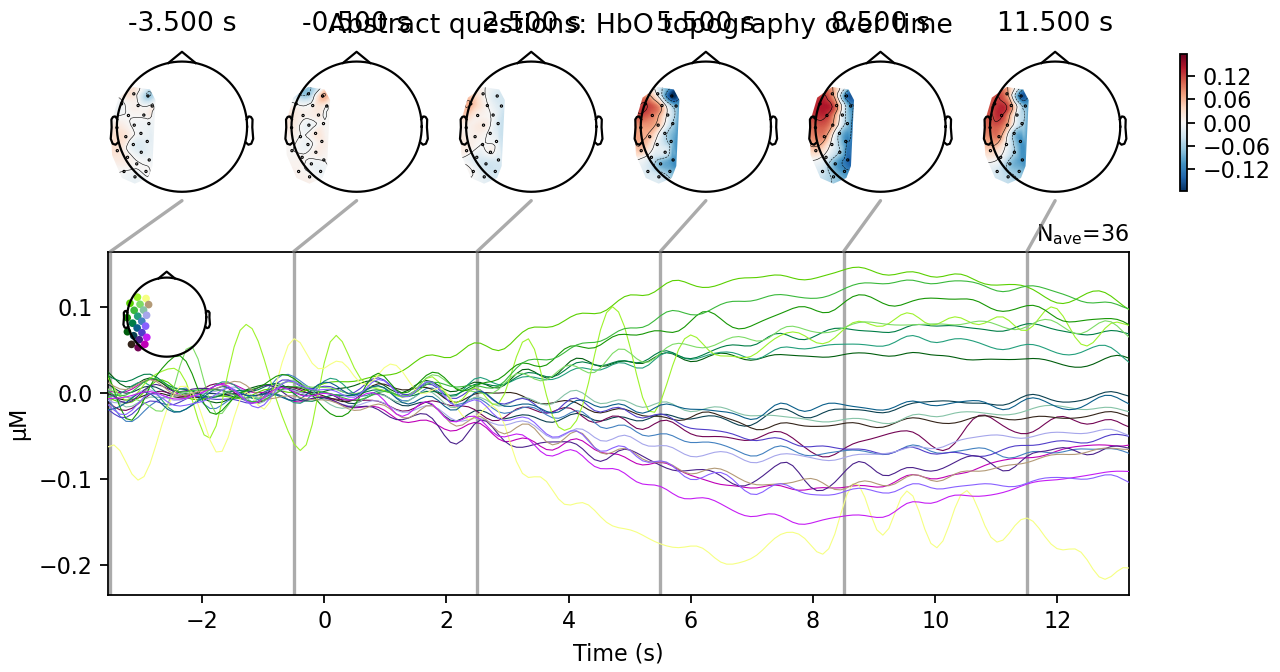
\includegraphics[width=0.95\linewidth]{../../figures/step5_visualization/abstract_hbo_joint.png}
\caption{Grand-average HbO topography over time for Abstract questions using the Step~5 included trial set.}
\end{figure}
\begin{figure}[H]
\centering
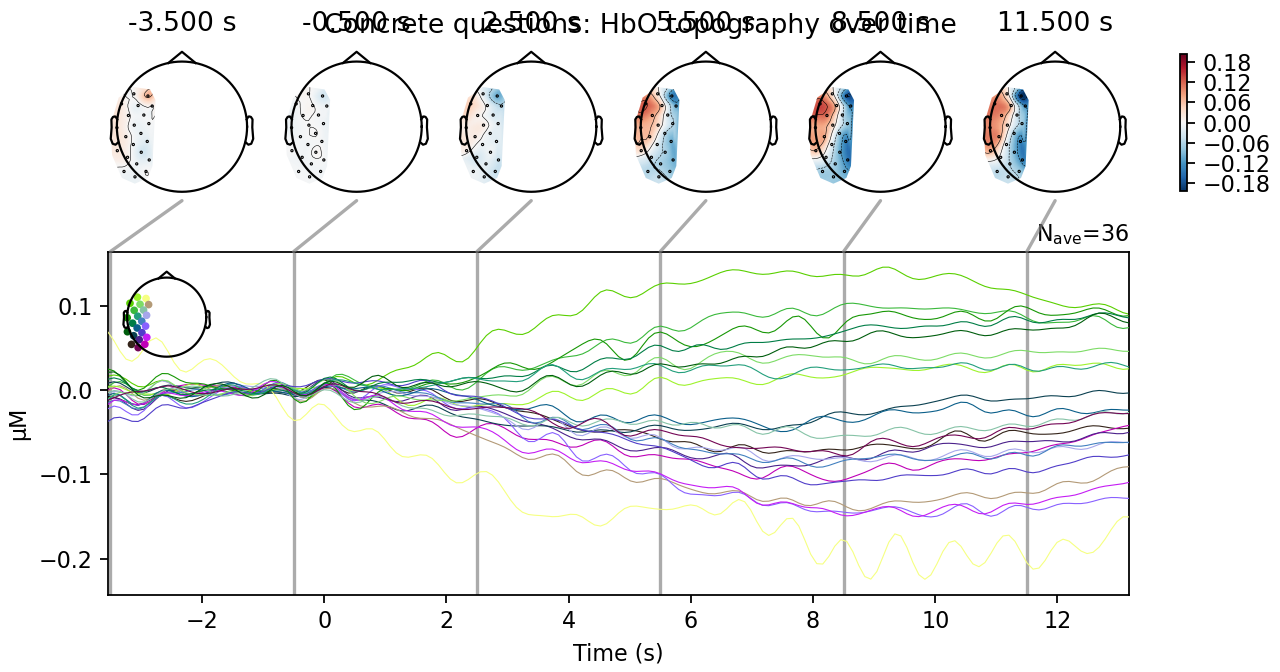
\includegraphics[width=0.95\linewidth]{../../figures/step5_visualization/concrete_hbo_joint.png}
\caption{Grand-average HbO topography over time for Concrete questions using the Step~5 included trial set.}
\end{figure}
\begin{figure}[H]
\centering
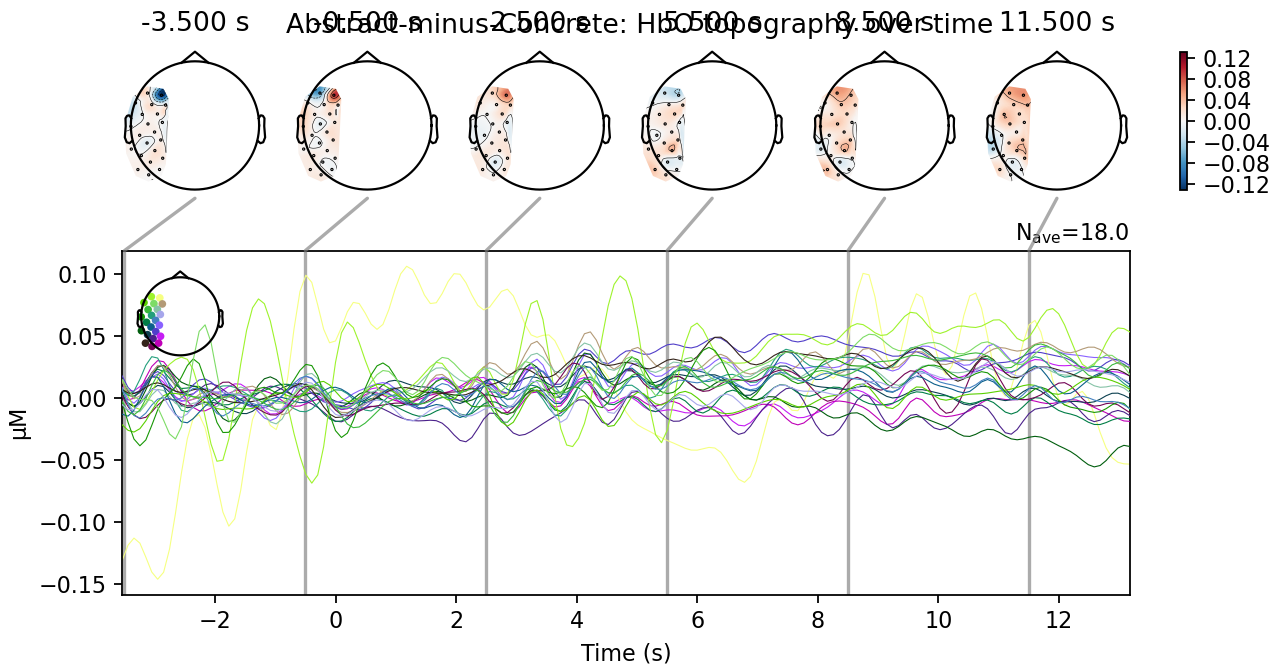
\includegraphics[width=0.95\linewidth]{../../figures/step5_visualization/abstract_minus_concrete_hbo_joint.png}
\caption{Grand-average Abstract-minus-Concrete HbO topography over time.}
\end{figure}
\subsection*{Condition Topomap Series}
\begin{figure}[H]
\centering
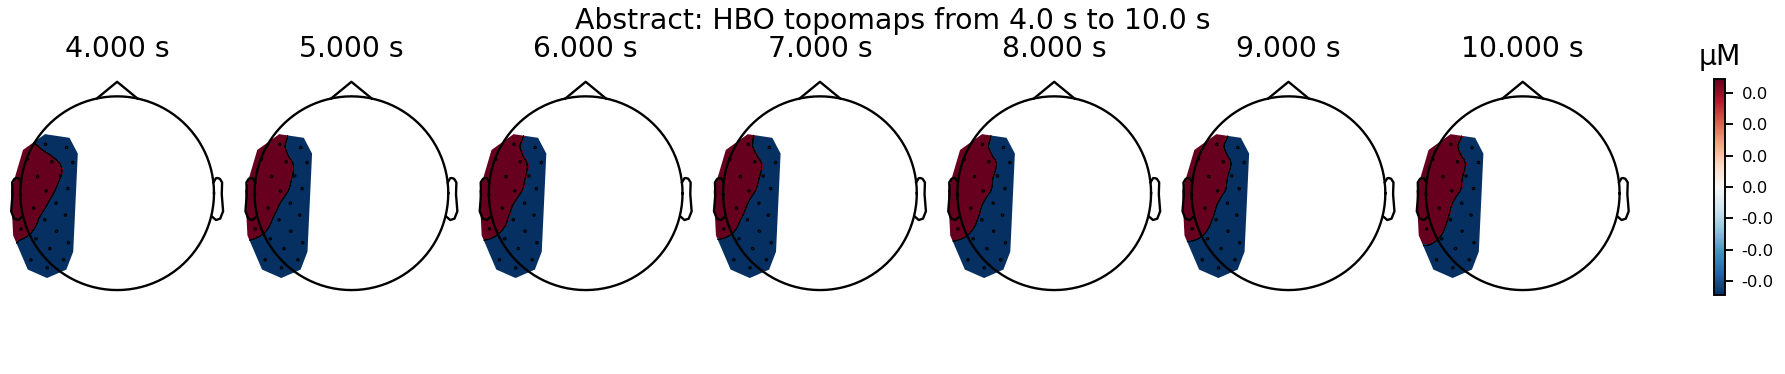
\includegraphics[width=0.48\linewidth]{../../figures/step5_visualization/abstract_hbo_topomap_series.png}
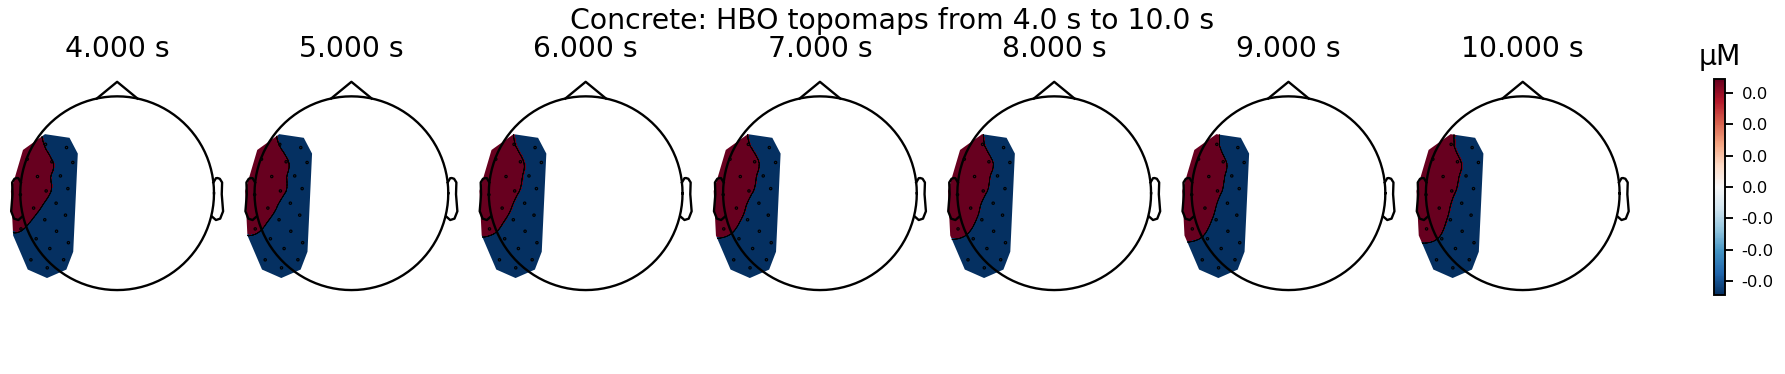
\includegraphics[width=0.48\linewidth]{../../figures/step5_visualization/concrete_hbo_topomap_series.png}
\caption{HbO topographic time series from 4.0~s to 10.0~s for the Abstract and Concrete conditions.}
\end{figure}
\begin{figure}[H]
\centering
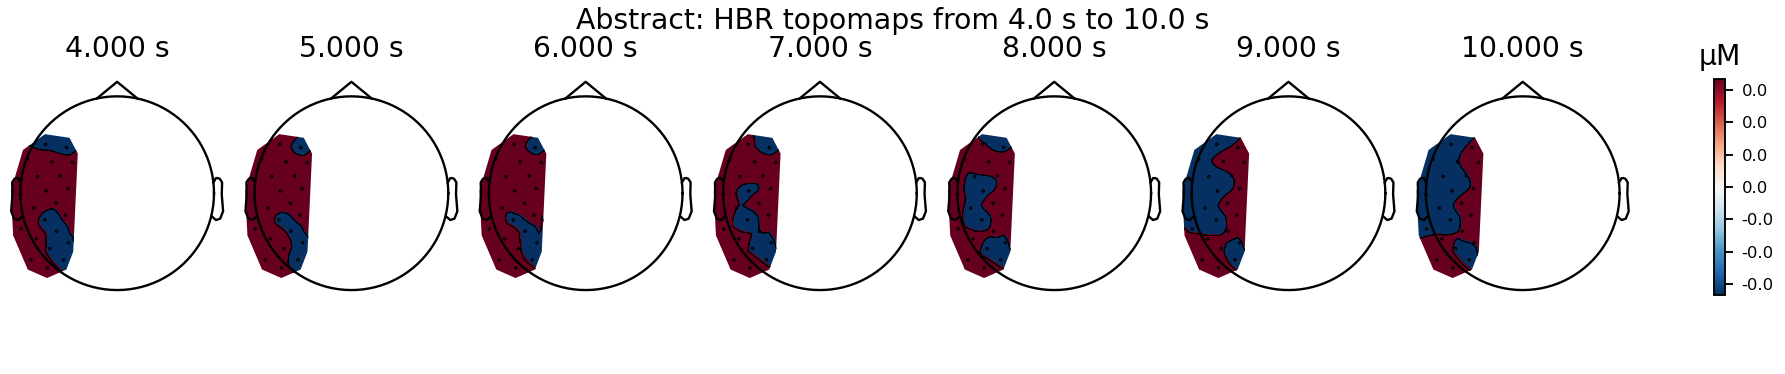
\includegraphics[width=0.48\linewidth]{../../figures/step5_visualization/abstract_hbr_topomap_series.png}
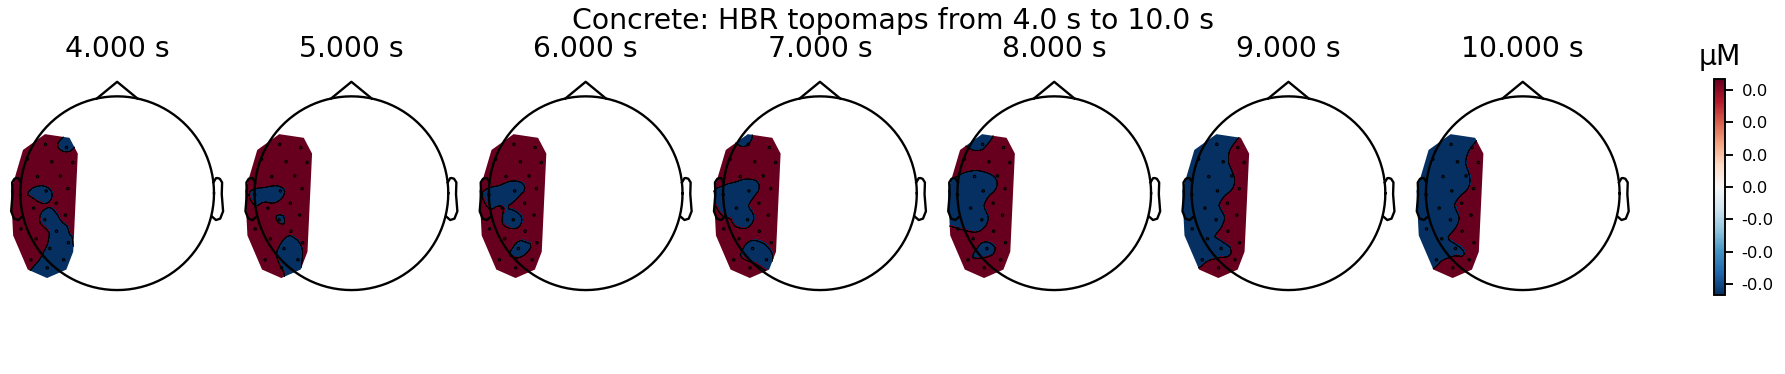
\includegraphics[width=0.48\linewidth]{../../figures/step5_visualization/concrete_hbr_topomap_series.png}
\caption{HbR topographic time series from 4.0~s to 10.0~s for the Abstract and Concrete conditions.}
\end{figure}
\subsection*{Single-Time Condition Comparison}
\begin{figure}[H]
\centering
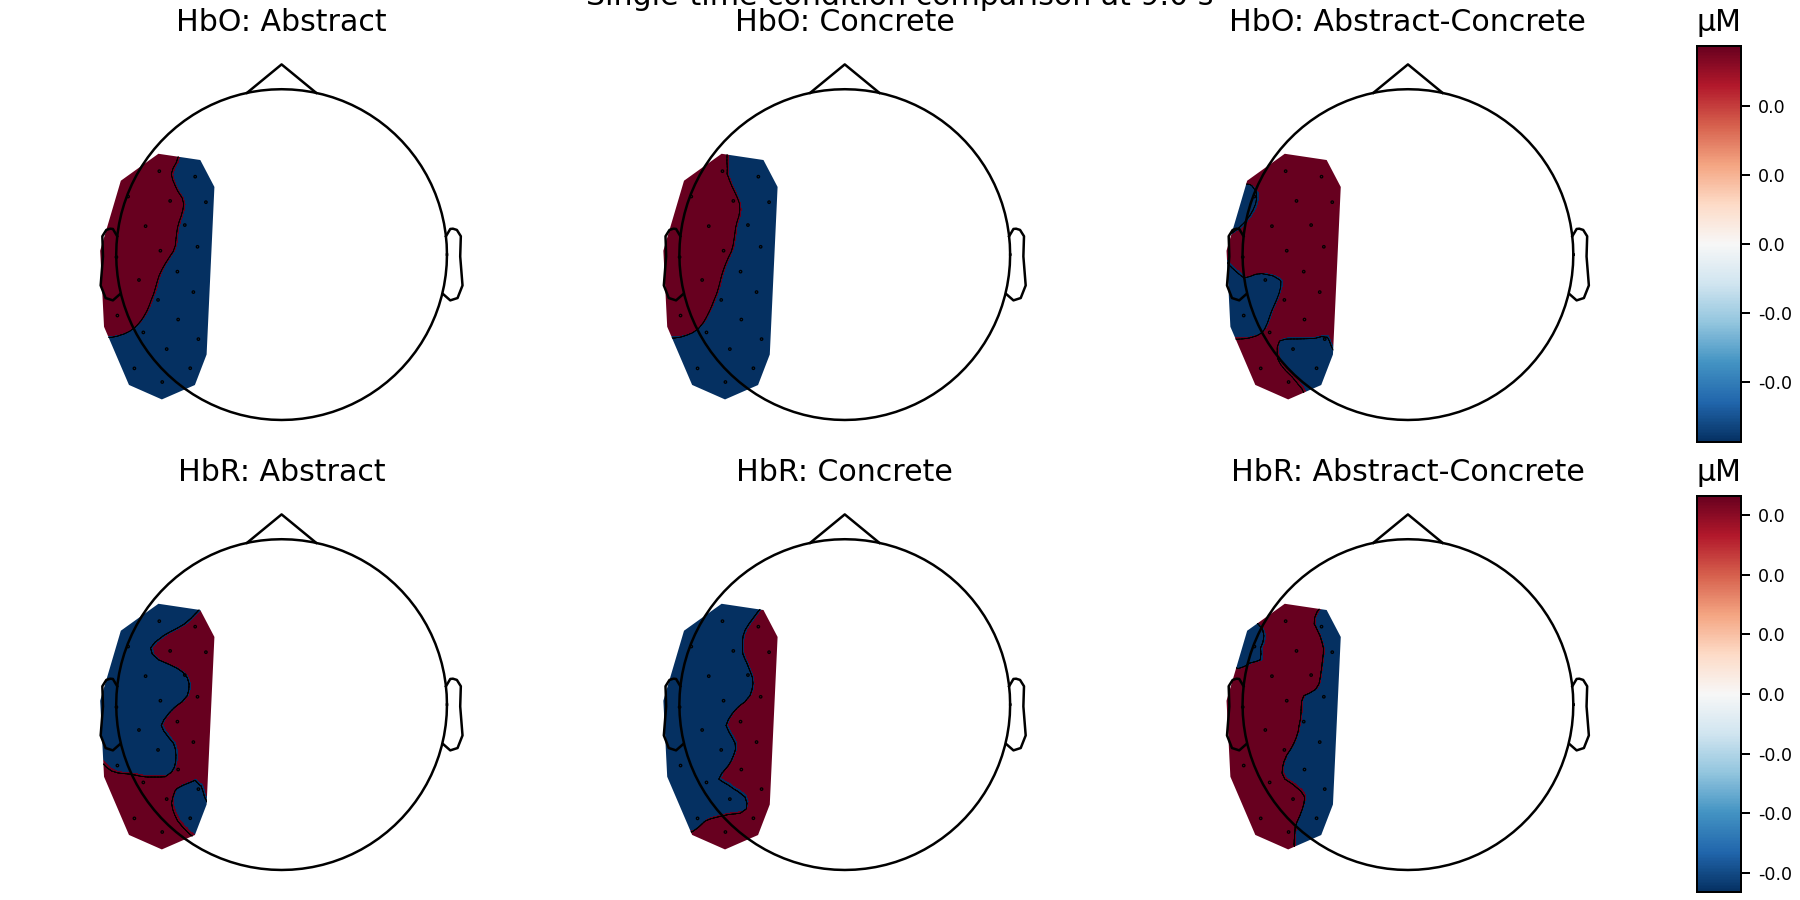
\includegraphics[width=0.95\linewidth]{../../figures/step5_visualization/abstract_concrete_single_time_comparison.png}
\caption{Single-time comparison at 9.0~s for Abstract, Concrete, and Abstract-minus-Concrete topographies for both HbO and HbR.}
\end{figure}
\subsection*{Channel-Wise Waveform Topography}
\begin{figure}[H]
\centering
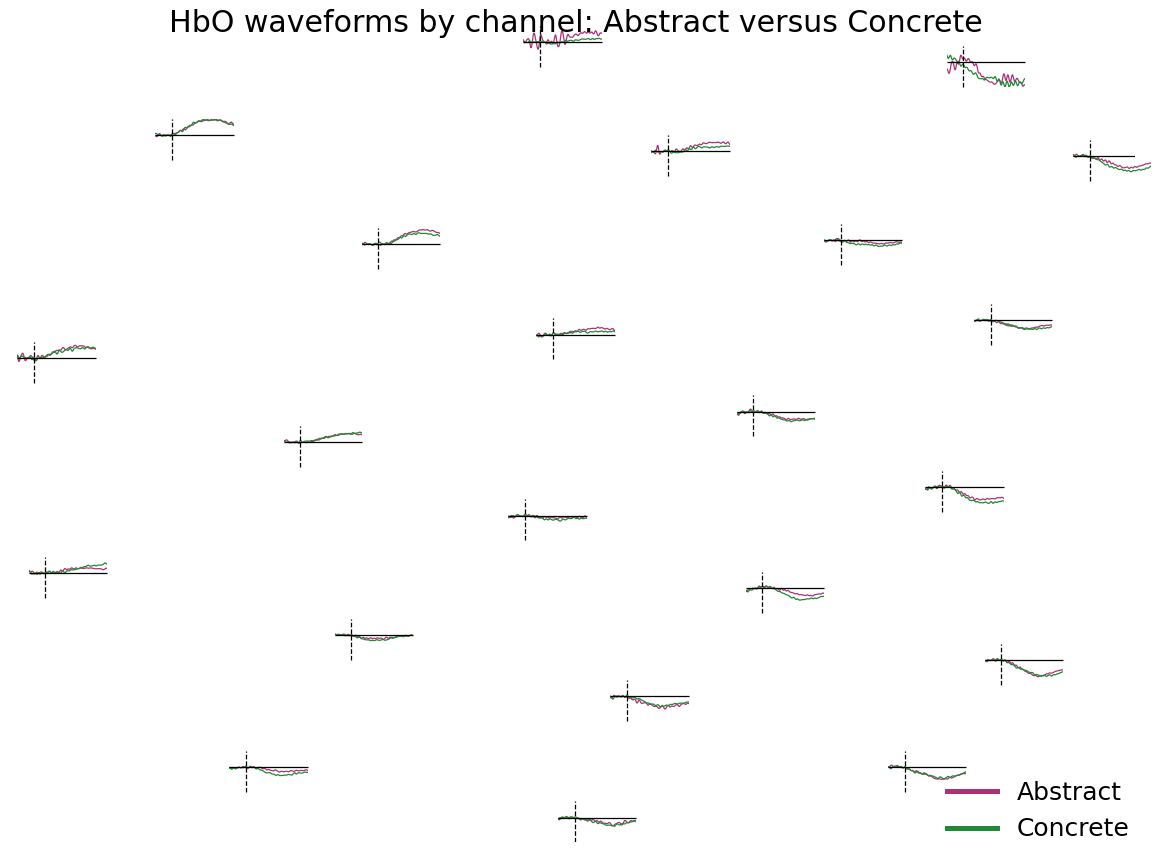
\includegraphics[width=0.95\linewidth]{../../figures/step5_visualization/abstract_concrete_hbo_evoked_topo.png}
\caption{HbO waveforms by long channel, overlaid for Abstract and Concrete, to show which local waveforms drive the descriptive topographic differences.}
\end{figure}
\end{document}
